\chapter{Artificially Simulate Jitter}\label{appendix:artificial_jitter}

%\lstset{language=Python}

In order to analyse the behaviour of the techniques studied in this thesis over misaligned side-channel traces, we simulated sometimes a jitter effect to misalign some well-synchronized traces in a controlled way. When jittering is present, the clock stability is altered and clock cycles are sampled by a varying number of time samples. To simulate such effect, the windows containing clock patterns of an acquisition are selected one by one and passed as input to the following function, described in python code, in charge to enlarge or reduce them in a random way. The randomness depends on two parameters \texttt{sigma} and \texttt{B}, being the number of inserted or removed points be almost normally distributed, with standard deviation given by \texttt{sigma}, but bounded. The bound is controlled by \texttt{B} by the following rule: the final size of a window has to be at least $\frac{1}{\text{\texttt{B}}}$ times the original size and at most \texttt{B} times the original size. The value assigned to newly inserted points is the linear interpolation of the previous and the following points.

\begin{lstlisting}[frame=single]
def enlarge_reduce_window(window,sigma,B): 
    Npts = window.shape[0]
    new_window = np.copy(window)
    deltaPts = int(np.floor(np.random.randn(1)[0]*sigma))
    if (deltaPts >= 0):
        deltaPts = min(Npts*(B-1),deltaPts)
        for i  in range(deltaPts):
            curr_size = new_window.shape[0]
            pos = int(np.floor(np.random.rand(1)*curr_size))
            if pos==0 or pos==curr_size-1:
                new_window = np.insert(new_window,
                 pos,new_window[pos])
            else:
                new_window = np.insert(new_window,pos, 
                (new_window[pos-1]+
                new_window[pos])/2.0)
    else:
        deltaPts = max(-Npts*(1-1/B),deltaPts)
        for i in range(-deltaPts):
            curr_size = new_window.shape[0]
            pos = int(np.floor(np.random.rand(1)*curr_size))
            new_window = np.delete(new_window,pos)
    return new_window
    
\end{lstlisting}

This deformation is applied to each clock pattern independently. We remark that is implies that, for example, The 19th clock cycle of a deformed acquisition suffers from the cumulation of the previous 18 deformations. For the sake of visualizing the effect of such a jitter simulation, in Fig.~\ref{fig:jitter_traces} we depict some traces of  \emph{DS\_low\_jitter} and of the \emph{DS\_high\_jitter} datasets, used for experiments in Sec~.\ref{sec:hardware}. They are obtained by perfectly synchronous acquisitions, with parameters set to \texttt{sigma} $= 2$, \texttt{B}$= 2$ for the \emph{DS\_low\_jitter}  dataset and \texttt{sigma} $= 6$, \texttt{B}$= 6$ for the \emph{DS\_high\_jitter} one.

\begin{figure}
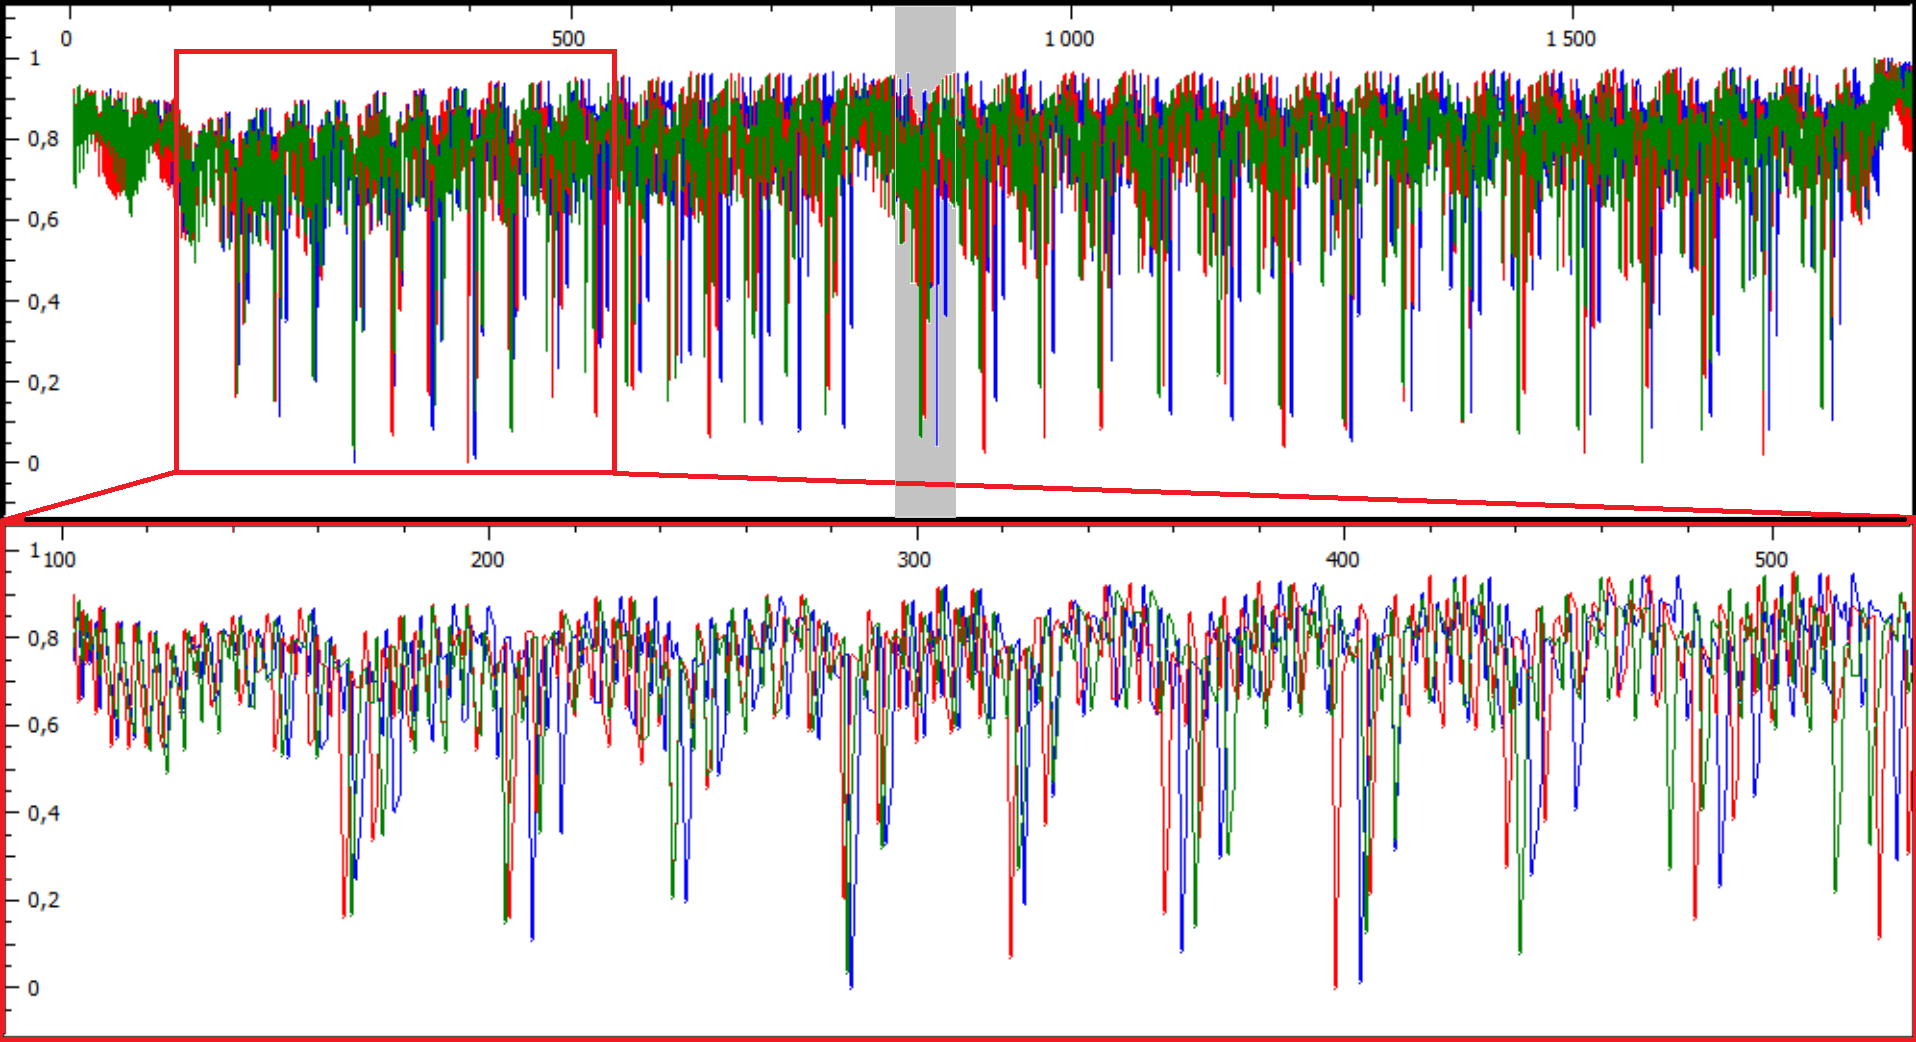
\includegraphics[width=.5\textwidth]{../Figures/CHES2017/jitter_2_2_framed.png} 
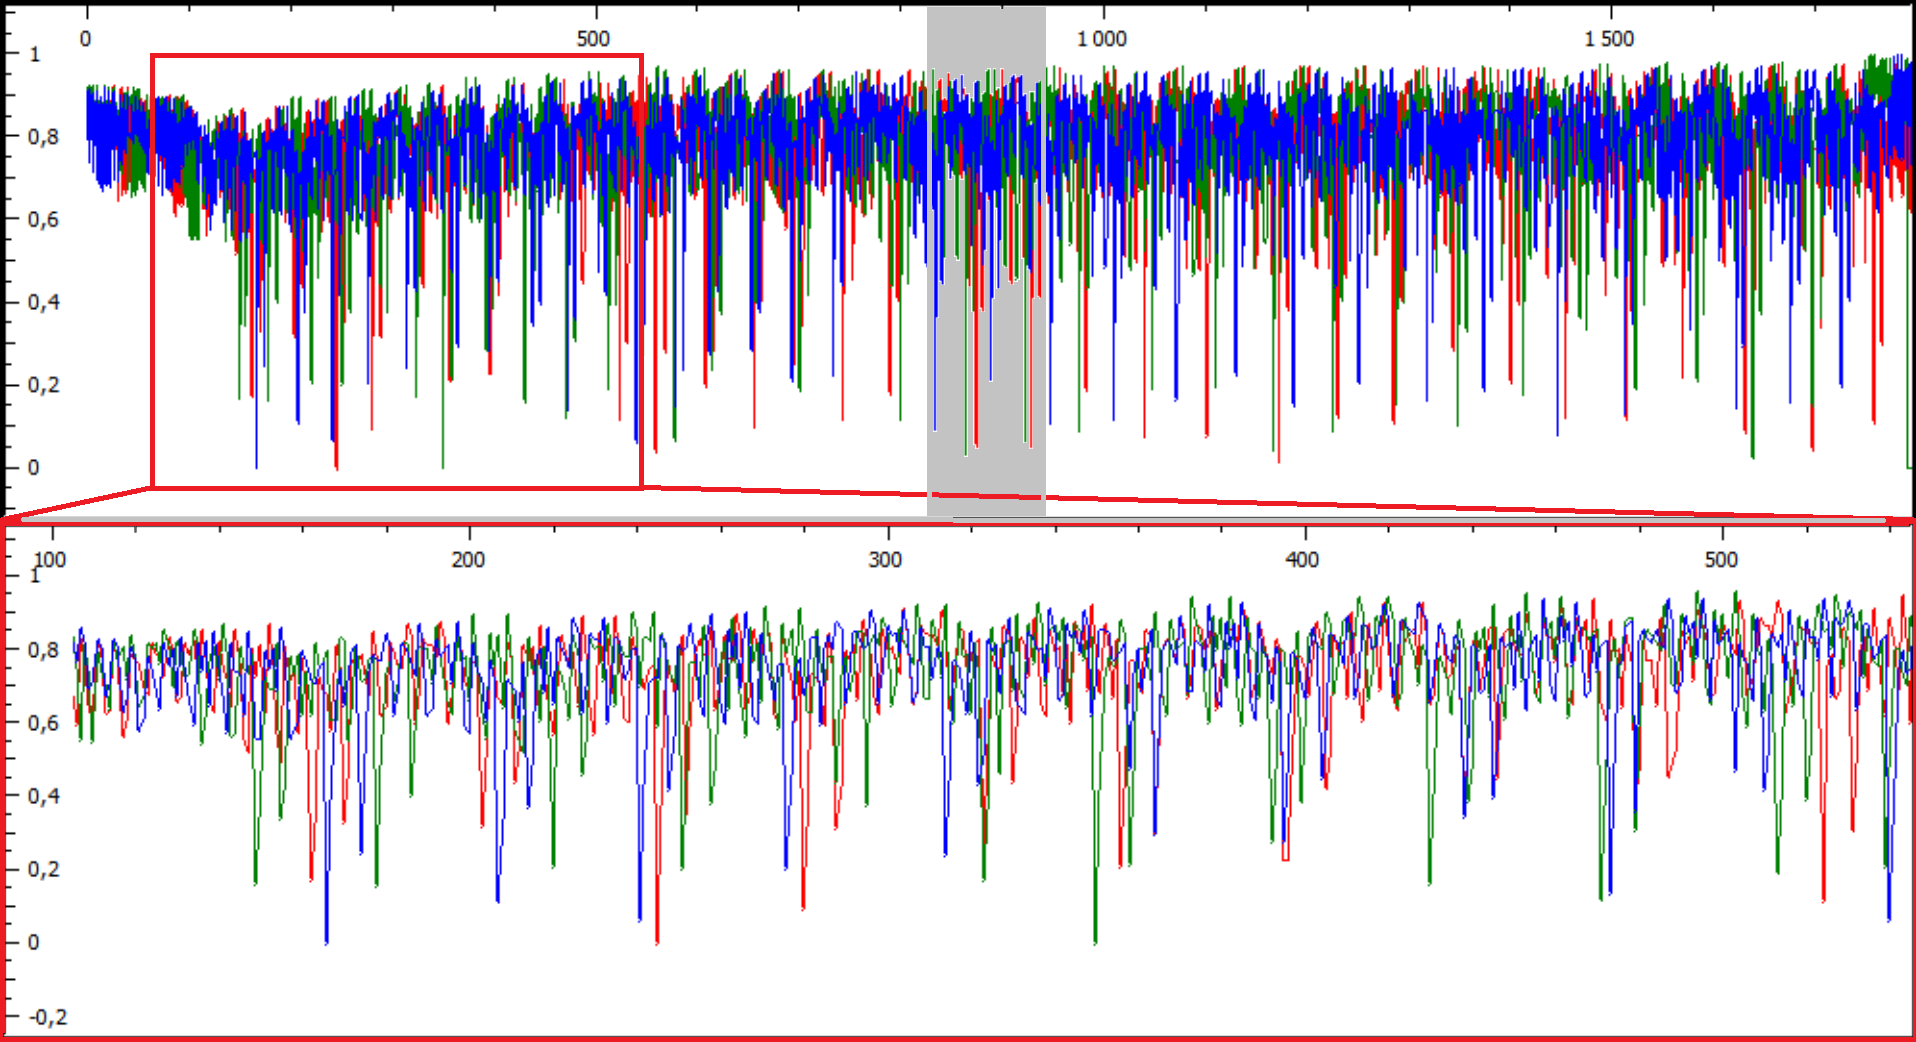
\includegraphics[width=.5\textwidth]{../Figures/CHES2017/jitter_6_6_framed.png} 
\caption[]{Left: some traces of the \emph{DS\_low\_jitter} dataset, a zoom of the part highlighted by the red rectangle is given in the bottom part. Right: some traces (and the relative) of the \emph{DS\_high\_jitter} dataset. The interesting clock cycle for experiments in Sec.~\ref{sec:hardware} is highlighted by the grey rectangular area.}\label{fig:jitter_traces}
\end{figure}


